\documentclass[journal,transmag]{IEEEtran}

% ..........................................................................
% Packages, configuration settings, and macro definitions.

\usepackage[pdftex]{graphicx}
\graphicspath{figures}
\DeclareGraphicsExtensions{.pdf,.jpeg,.png}

\usepackage[pdftex,rgb,dvipsnames,svgnames,hyperref,table]{xcolor}

\usepackage[pdftex,breaklinks=true,colorlinks=true,
	bookmarks=false,pdfhighlight=/O,
	urlcolor=DarkBlue,citecolor=DarkRed,linkcolor=DarkBlue]{hyperref}

\usepackage[cmex10]{amsmath}
\interdisplaylinepenalty=2500

\usepackage{amssymb}
\usepackage{amsfonts}
\usepackage{multicol}
\usepackage{enumitem}
\usepackage{accsupp}
\usepackage{array}
\usepackage[caption=false,font=footnotesize]{subfig}
\usepackage{booktabs}
\usepackage{xspace}
\usepackage{soul}
\usepackage{url}
\usepackage{hyphenat}
\usepackage[english]{babel}

% Correct bad hyphenation here
\hyphenation{op-tical net-works semi-conduc-tor ana-ly-tics}

\usepackage{pdfcomment}
\newcommand{\comment}[3]{\pdfmarkupcomment[markup=Highlight,color=yellow,author={#2}]{#1}{#3}}

% ..........................................................................
% Body.

\begin{document}

\markboth{IEEE Transactions on Biomedical Engineering}{2015 whole-cell modeling summer school meeting report}

\title{Combining standards for tomorrow's models: Report of the 2015 whole-cell modeling summer school}

\author{
	\IEEEauthorblockN{
		Dagmar Waltemath\IEEEauthorrefmark{1},
		Falk Schreiber\IEEEauthorrefmark{2}, 
		Jonathan R. Karr\IEEEauthorrefmark{3}, and
		Other People
	}
	
	\IEEEauthorblockA{\IEEEauthorrefmark{1}University of Rostock}
	\IEEEauthorblockA{\IEEEauthorrefmark{2}Faculty of IT, Monash University}
	\IEEEauthorblockA{\IEEEauthorrefmark{3}Department of Genetics \& Genomic Sciences, Icahn School of Medicine at Mount Sinai} 
	%New York, NY 10029 USA\\Email: \href{mailto:karr@mssm.edu}{karr@mssm.edu}}
	
	\thanks{Corresponding author email: dagmar.waltemath@uni-rostock.de}
}

\IEEEtitleabstractindextext{
	\begin{abstract}
	Computational modeling is an increasingly powerful and important tool for biological discovery, bioengineering, and medicine. 
	Recently, researchers developed the first whole-cell computational model which represents every individual gene.
	However, significant work remains to develop fully complete and accurate models of cells. 
	We organized the 2015 whole-cell modeling summer school to teach students the latest cell modeling methods, as well as to bring the computational systems biology community together to assess the need and limitations of our current standards for whole-cell modeling.
	We found that a whole-cell modeling standard would accelerate the development of whole-cell models, and that more work is needed to expand our current standards to support whole-cell models.
	% One major criticism of these standards is that they lag behind current developments and thereby may not be suitable to fully encode today's models. To overcome this problem, the applicants, under the guidance of the COMBINE effort, will organize a summer school for standard developers and modelers, i.e., users of these standards. The main goal is to explore the expressivity of current standard formats using the example of the famous whole-cell model, which has not yet been encoded in a standard format.
	\end{abstract}
	
	% Note that keywords are not normally used for peer review papers.
	\begin{IEEEkeywords}
	Whole-cell modeling, Systems biology, Simulation, Computational modeling, Standards, Education
	\end{IEEEkeywords}
}

\maketitle
\IEEEdisplaynontitleabstractindextext
\IEEEpeerreviewmaketitle

\section{Introduction}

% The very first letter is a 2 line initial drop letter followed by the rest of the first word in caps.
% 
% form to use if the first word consists of a single letter:
% \IEEEPARstart{A}{demo} file is ....
% 
% form to use if you need the single drop letter followed by normal text (unknown if ever used by IEEE):
% \IEEEPARstart{A}{}demo file is ....
% 
% Some journals put the first two words in caps:
% \IEEEPARstart{T}{his demo} file is ....
% 
% Here we have the typical use of a "T" for an initial drop letter and "HIS" in caps to complete the first word.
% is a report of the VW Whole-cell Summer School held in Rostock during April, 2015.

\IEEEPARstart{R}{esearch} in the life sciences is increasingly computational, and computational modeling is a promising tool for biological discovery, bioengineering, and medicine. Computational modeling has already been used to identify new metabolic genes~\cite{Reed2006}, add metabolic pathways to bacteria~\cite{Lee2009}, and identify potential new antimicrobial drug targets~\cite{Lee2012}. 
Computational models also have the potential to enable bioengineers to design entirely new strains of bacteria optimized for industrial tasks such as chemical synthesis, biofuel production, and waste decontamination, as well as to enable clinicians to design individualized medical therapies tailored to each patient's unique genome. 
Realizing this potential requires more comprehensive and accurate computational models which are capable of predicting cellular behavior from genotype, but also standardized ways to exchange model description, modeling parameters as well as model visualizations~\cite{Macklin2014,Karr2015,Klipp07}.

Recently, researchers at Stanford University developed the first whole-cell model of the gram-positive bacterium \textit{Mycoplasma genitalium}~\cite{Karr2012}. 
The model represents the entire life cycle of a single cell including the copy number of each metabolite, RNA, and protein species, and it accounts for every known gene function. 
The model is comprised of multiple sub-models, each of which was implemented using different mathematical representations such as ordinary differential equations (ODEs), flux balance analysis (FBA), and Boolean rules (BRs) and trained using different experimental data. 

The \textit{M. genitalium} whole-cell model was implemented in MATLAB, is available open-source under the MIT license, and was extensively documented. 
This has enabled other researchers to expand the model and use it for their own research, as well as use it as a teaching tool in systems biology courses in universities across the world. 

Although MATLAB is commonly used by academic researchers, it is proprietary and expensive. In addition, because many of the biological details of the model are intertwined with the MATLAB code, significant domain expertise is required to understand, modify, and expand the model. 
A more transparent, standardized implementation is needed to enable more researchers to use the existing whole-cell model, as well as to contribute to whole-cell modeling. 
In turn, this would enable researchers to develop faster and more efficient whole-cell model simulators, more deeply explore whole-cell model predictions, and more rigorously evaluate whole-cell models; thereby accelerating the whole-cell modeling field.

The COmputational Modeling in BIology NEtwork (COMBINE)~\cite{le2011meeting} is the umbrella organisation for various standardization initiatives in computational biology and beyond.
It provides  to the community a set of data formats that allow software tools to exchange models (in SBML~\cite{hucka2003} or CellML~\cite{hedley_2001b}), simulation experiment descriptions (in SED-ML~\cite{sedml2011}), maps (in SBGN-ML~\cite{IerselVCBBLDSDMFAMMKNS12}), and even reproducible simulation setups (as COMBINE Archives \cite{Bergmann2014combine}).  
% We used standard formats using open standards (COMBINE standards) and open software (COMBINE-compliant software)., including SBML~, CellML~\cite{hedley_2001b}, SED-ML~\cite{sedml2011}, and SBGN~\cite{LeNovereHMMSS09}. 
% All formats are \textit{de facto} standards. 
% SBML represents networks in biology; CellML represents networks in physiology; SED-ML encodes simulation descriptions; and SBGN encodes the graphical representation of networks. 
Together, these standards allow for the encoding of virtual experiments in biology. 
Many so-called COMBINE-compliant software exist to run these experiments. 

The Systems Biology Markup Language (SBML) and the Cell Markup Language (CellML) are the most commonly used systems biology modeling standards. 
Both languages can be used to develop a wide variety of models including ODEs, logical, and FBA models, and both have been used to build hundreds of models. 
However, neither language supports several of the features needed for whole-cell modeling including large, sparsely occupied state spaces and multi-algorithm simulations. 
In addition, the System Biology Graphical Notation (SBGN)~\cite{LeNovereHMMSS09} is the language to encode the visual representation of a model, but has currently also restrictions regarding the visualization of whole-cell models. 
Consequently, further work is needed to expand the SBML, CellML, and SBGN languages to support whole-cell models.

To analyse the shortcomings of current standards for whole-cell modeling, we organized the \emph{2015 whole-cell modeling summer school}. 
The summer school aimed to train students in whole-cell modeling, as well as to initiate the further development of the SBML and SBGN languages to support whole-cell modeling.  
The goals of the school were three-fold: 
First and foremost, the goal of the course was to train young researchers how to build whole-cell models, how to develop sub-models of individual cellular pathways using different mathematical formalisms and encode them using SBML and graphically encode them using SBGN, and how to combine sub-models into a single model. 
The second goal of the course was to identify the features that must be added to the SBML and SBGN languages to support whole-cell models, and state-of-the-art models in general. 
The third goal of the course was to initiate the recoding of the \textit{M. genitalium} whole-cell model into SBML and SBGN.

Here, we summarize the educational and scientific outcomes of the summer school. The paper is structured as follows: 
Section II deals with the format of the summer school.
Section III presents the results achived.  
Section IV shows the lessons we learned from the summer school, specifically  the limitations of SBML and SBGN. 
Section V discusses future directions. 
We finish with a conclusion in Section VI. 

\section{The 2015 whole-cell modeling summer school}

The idea for this summer school was born at the 2012 COMBINE meeting~\cite{COMBINE2012} in Toronto. During that meeting, the first COMBINE tutorial took place. It was intended at modelers working with COMBINE standards and COMBINE-compliant software tools. 
While the tutorial room was full, a short survey revealed that not many modelers were actually participating.  
This  led to a longer discussion about how to best reach the end-users of the COMBINE standards. 
During that discussion, the idea of a summer school on translating a famous model into a COMBINE-compliant representation was born. 
Two years later, the Volkswagen Foundation funded this idea. 

We selected 10 tutors to support us in preparing and organising the event. 
Among the applicants, we selected 50 students  who joined us in a week of hacking and coding, exploring the whole-cell model, networking and learning more about the importance of reproducible science.

The goal for the summer school was to re-build the Karr model using only standard representation formats and open software tools. 
This ambitious goal demanded much work ahead of the summer school itself:  
In preparation of the summer school the tutors decomposed the model into modules (consisting of one or a few submodels of the initial model). We assigned the students to eight research groups, each led by a tutor and each \comment{responsible for one module}{Waltemath}{We could add the overview figure of the Karr model here, split into the eight submodules; or we could add the overview of all groups and participants here, but maybe this is a bit too unusual?}.  
During  meetings through Google hangout and using code sharing through GitHub,  students got used to the MATLAB whole-cell model and started to think about their specific modul, especially the interfaces. 
The groups got to know each other and distributed the preparatory tasks, discussed the software tools they intended to use and planned their workshop days. 
 
The summer school week itself was structured in two invited talks, daily working sessions, a daily wrap-up (summary) presentation of each working group, a poster session, and a final presentation of results on the last day.

\subsection{Invited talks}
Two scientific invited talks were held at the summer school. 
The first speaker was Dr. Michael Hucka from the California Institute of Technology, USA. 
He provided an overview of the COMBINE initiative, COMBINE standards and tools supporting these standards. 
His talk focused on the formats most relevant to whole-cell modeling. 
% Dr. Hucka is one of the founders of SBML and COMBINE.

The second speaker was Dr. Jonathan Karr from the Icahn School of Medicine at Mount Sinai School, USA. 
He  provided overviews of the whole-cell modeling field, of his own research toward developing and applying whole-cell models for scientific discovery and engineering, and of the \textit{M. genitalium} whole-cell model which he and his colleagues recently developed.
Dr. Karr concluded his talk by outlining several research projects which his own group is pursuing to expand the scope of whole-cell models and use whole-cell models to engineer faster growing bacteria.
% Dr. Karr's inspiring talk set the basis for re-coding his model.

\subsection{Daily working sessions}
The working sessions ran from Tuesday until Friday. 
The goal of each team was to provide a running module of their part of the model, together with the necessary inputs and outputs (interface) for the other groups. 

Each day started with a plenary session, which summarized the goals for the day. 
The remaining time, students worked in their own groups of five to seven people, working on their single modules. 
Two additional groups were formed to coordinate on the meta-level: 
The Integration group developed an integration mechanism for the single modules, using the software iBioSim~\cite{Stevens2013}. 
They defined the interfaces between modules, how to select processes, and they discussed how to run the model as a whole.
The Floating group consisted of experts in specific areas needed by all other groups.
For example, Jonathan Karr visited every group to advise on the biology and modeling part. 
Falk Schreiber visited the groups to discuss issues with the SBGN representations of the model. 

It was very  interesting to observe how the single groups  approached the general problem of converting an existing model into a COMBINE-compliant representation. 
Some groups started by reading the supplemental material and drawing an SBGN map from that, using software tools such as  Cell Designer \cite{funahashi2008celldesigner} or VANTED~\cite{Rohn2012}. 
Based on the SBGN-ML code they then scripted a transformation into SBML. 
Other groups started by going through the MATLAB code and converting it into SBML, and from there into SBGN. 
Other teams rebuilt the model directly in software tools such as  COPASI~\cite{Mendes2009} or BioUML~\cite{Kolpakov2006}, again based on the original publication.  

% Popular software, used during the summer school, are COPASI~\cite{Mendes2009}, BioUML~\cite{Kolpakov2006}, VANTED~\cite{Rohn2012}, and iBioSim~\cite{Stevens2013}.
Each day closed with  a plenary session where the single groups presented their results of the day and got feedback from the whole group. In addition, further topics for discussion were planned.
Throughout the workshop, each student presented at least once.  

Additionally, we arranged for spontaneous discussion rounds whenever problems occurred in more than one team. 
For example, many groups needed to represent DNA binding sites in SBML. 
The XML code of the SBML got very large when trying to represent every possible state of the system at each time point. 
Therefore, a break out session was organized that discussed the various solutions. 

\subsection{Poster session}
The poster session enabled participants to present their own research. 
27 students presented posters. Many of the students presented projects on whole-cell modeling or other computational systems biology projects.

\section{Results}

\subsection{Educating young systems biologists}
One of the major intentions of this summer school was to educate young scientists. 
The whole-cell model is now one of the standard models in computational biology. 
It is therefore  important for researchers to be informed about the model, its capabilities, the insights it gives and how it can be used and reused. 

Although we made sure during the selection process that the students had some knowledge in modelling and some of the standards, they had very different backgrounds from computer science to biology, and hence different knowledge regarding modeling, programming, systems biology and standards. Therefore a special focus of the summer school was on making  the participants familiar with cell biology, common modeling methods (such as ODE, FBA, and BR), model integration, and modeling standards (SBML, SED-ML, and SGBN). Many students attended the pre-course classes via Google Hangouts, which already provided additional background towards the aims of the summer school. 
Prior to the course, most of the students had already run the whole-cell model. 

\comment{Text}{Waltemath}{Would like to ask Tom to help here, using the statistical data we have on background, degree of prior knowledge etc}
\comment{Text}{Karr}{elaborate on what computational systems biology knowledge students already had: (1) modeling, (2) programming, (3) systems biology, (4) standards}

After the summer school, many students reported that they learned a lot about using open-source modeling software. 
In particular, students reported increased understanding of SBML and SBGN, and better awareness of reproducibility issues.

The course was also a great networking event for both the students and tutors. 
Students had opportunities to connect with other young computational systems biology researchers from around the world.
The poster session provided students an opportunity to share their own work and get valuable feedback from each other, the tutors, and other scientists from the University of Rostock.
Several of the tutors advertised open positions in the labs, as well as upcoming courses and meetings including the April 2016 whole-cell modeling summer school which Jonathan Karr, Luis Serrano, Maria Lluch-Senar, and Javier Carrera are organizing in Barcelona, Spain.

% \subsection{\comment{Setting the goal}{Karr}{I would probably eliminate this section and merge the thoughts about code committed to GitHub with the following section. 
% If the goal was to create a working model, then the goal wasn't met and likely will never be met. Probably very few of the SBML sub-models actually work. 
% None of them have been tested to any degree. And a lot of work remains to integrate them. 
% I definitely wouldn't claim the sub-models will be published by the fall because this is not likely to happen.}}
% \comment{Setting the goal}{Waltemath}{Agreed}

% The goal to encode the whole-cell model was ambitious from the beginning, but the expectations have been more than met. 
% All participants dedicated their full time to working on the project, preparing initial results weeks beforehand, and even worked long hours. 
% The achieved results are of high quality and the spirit at the summer school was very positive over the whole week. 
% With 3 more days on the same project, we would have been able to test and then publish the 28 modules. 
% The final state after one week is that all material is there, but the modules need to be tested and integrated. 
% Several weeks after the summer school, the activity on the Git project is still high, and it can be expected that we will finish these two tasks before summer. 
% The modules shall be published in BioModels Database by autumn 2015. 

\subsection{Progress toward an SBML whole-cell model}
In addition to training young systems biology researchers, the course produced preliminary SBML and SBGN-ML encoded versions of each of the whole-cell models parts (submodels).
We developed 28  modules in COMBINE formats that represent the majority of the whole-cell model, and which can be run in open-source software.
An overview of progress in the single modules is shown in 
\comment{Table~1}{Waltemath}{Are we going to put the table here? We could state that the data was gathered through  self-evaluation within the single teams}. 
The sub-models are available open-source at \url{http://github.com/dagwa} and \url{https://github.com/whole-cell-tutors/wholecell}. 
The scientific community will benefit from these open-access, reusable versions of the sub-models that make up the model.

% TODO: Insert table of progress here

Further work is needed to finalize the modules and integrate these sub-models into a single model. 
We hope to achieve this over the next several months.

\section{Lessons learned}

\subsection{Limitations of SBML and SBGN for whole-cell modeling}
SBML and SBGN have never been applied before to such a large and complex model, and therefore using those standards for the whole-cell model provided interesting insights. 
Specific issues in SBML included:
\begin{itemize}
\item the representation of large, combinatorial state spaces (such as different states of the binding sites) summing up to over one million in the SBML file, 
\item the lack of representation of arrays in core SBML, 
\item the generation of random numbers, and 
\item the sharing of variables across modules. 
\end{itemize}
In SBGN specific issues included:
\begin{itemize}
\item the size and (automatic) layout of some diagrams and
\item the need to have mixed diagrams containing more than one SBGN language (SBGN has three sub-languages: Process description, Entity Relationship and Activity Flow).
\end{itemize}

A particular problem was the lack of concepts to represent large state spaces sparsely. Currently, SBML enforced the enumeration of the entire space, which is inefficient for combinatorially large spaces. A first improvement is the introduction of arrays, as suggested in the specification of the SBML Arrays package~\cite{SBMLArray}. However, arrays alone will not solve this problem. 
We faced serious problems in representing, for example, variations in DNA binding sites. 
While MATLAB does have concepts for the representation of arrays and vectors, SBML lacks comprehensive ways of encoding these. 
Here, the discussions between modelers, standard developers and tool developers were particularly interesting, as arguments were provided from very different view points.

\subsection{Interaction within groups and with the modeling community} 
We deliberately formed mixed groups of standard developers (mostly the tutors) with modelers (mostly the students). 
At the same time we arranged students in groups so that their expertise matched the specific module, and so that the groups themselves consisted of heterogeneous scientists in terms of education. 
Lastly, another aspect for building the groups was that we did not want the participants to know each other before to enhance the network experience for everybody and the internationality of the groups, whenever possible. 
The resulting groups thus were divergent in many aspects. 
The benefit of this divergence was that all participants trained their competences in interdisciplinary work, and the surrounding and the frame of the summer school led to a communicative environment. 

The positive effect on the standardization community became immediately visible:
throughout the summer school, the participants discussed features of existing standards, thereby providing feedback on the usability of COMBINE standards and associated software tools.
This feedback is going to be forwarded into the COMBINE community, for example through presentations at the annual community meetings COMBINE and HARMONY.

\subsection{Building a successful summer school}
From the feedback that we received, we conclude that the summer school was overall well perceived. 
There were many aspects which contributed to the success: 
\begin{itemize}
\item selection of team members (to ensure that there are no cliques within a team and that different backgrounds are available within each team), 
\item mentoring by expert-tutors (which are well established scientists in the field), 
\item flexibility in the schedule, 
\item daily wrap-ups to discuss the progress of the different teams, 
\item clear overall goals of the summer school,
\item generous financial support through the funding agency (which covered most to all of the costs of the students and tutors), and 
\item social activities during the summer school.
\end{itemize}
Most participants thought that it was an unusual format for  a summer school, but that this gave them the opportunity to learn a lot. 
However, two participants mentioned that they had not been satisfied with the format, as they would have wished for a tighter schedule with more lectures. 

\section{Future steps}

The summer school was only a first step towards accelerating the development of whole-cell models. 
As outlined above, there are several areas to continue: further education of scientists in modeling methods and modeling standards, further development of standards for models, and -- related to the model of \textit{Mycoplasma genitalium} -- finalizing the moduls and their integration to obtain the first whole cell model encoded in SBML and SBGN, which should be published in the BioModels database~\cite{li2010biomodels}. 

The participants of the summer school plan to continue working in their  groups even after the close of the school. 
Specifically, the groups will meet virtually via Google Hangouts, to finalize the representation of the modules, the annotations, and the graphical maps. 
We will continue the project in a second Whole-Cell workshop, which takes place as a satellite meeting to the 2015 COMBINE conference in Salt Lake City, October 2015.

In addition, lessons learned from the summer school and weaknesses of COMBINE standards are scheduled for the 2015 standardization meetings HARMONY and COMBINE.  It will therefore foster further standard development in systems biology. 

\section{Conclusion}
Computational modeling is increasingly important for biological discovery, bioengineering, and medicine, and whole-cell models are expected to become a standard in the future. 
The whole-cell modelling summer school targeted this critical area and  provided  training to young researchers how to build whole-cell models (including how to develop sub-models, encode them using SBML and SBGN, and  combine them into a single model), identified features that must be added to the SBML and SBGN languages to support  whole-cell models, and initiated the recoding of the \textit{M. genitalium} whole-cell model into SBML and SBGN.

The close connection between tool developers, standard developers, and modelers is essential and yet usually missing. 
The single communities have their own meetings and it happens that the communication between them is rather sparse. 
This summer school, however, offered a new channel of communication, through a very concrete task. 
The fact that modelers openly and directly pointed at lacks in existing standards, and that this criticism was converted into positive action on the developers site is for us the biggest achievement of the summer school. 
We hope that the summer school will inspire more events like this, where modelers and standard developers work together to solve a biological problem.

The experiences of this summer school will be reported at this year's HARMONY and COMBINE meetings (as invited talks, opening the two major standardisation meetings for
systems biology). 
We also aim to give feedback through our European networks, such as EraNet SysBio \cite{ERASysBio2015}, CaSYM \cite{CaSYM2015} and ISBE \cite{Wolkenhauer2009}.
Jonathan Karr furthermore announced another summer school on whole-cell models, taking place in Barcelona in 2016, but with a focus on the theory behind modeling whole cells.

We believe that this summer school set the path for a new series of meetings related to whole-cell modeling.
Lastly, we hope that this summer school will become a prime example for modern educational events, showcasing how standard development can happen in close interaction with the end-users.

At the final plenum, all tutors agreed that the goals of the summer school could not have been achieved without the interdisciplinary mix of expertises. 
The interdisciplinarity helped to see the task from different angles, and certainly it allowed us to try very different approaches to solving a problem (from brute force, to working with design thinking methods). 
In the opening to the summer school we spoke of the effect of swarm intelligence, and this is what happened during the week of work.

\section*{Acknowledgment}
The course was supported by a grant from the Volkswagen Foundation to DW and FS. 

\ifCLASSOPTIONcaptionsoff
  \newpage
\fi

\bibliographystyle{IEEEtran}
\bibliography{IEEEabrv,report}

% biography section
% 
% If you have an EPS/PDF photo (graphicx package needed) extra braces are needed around the contents of the optional argument to biography to prevent
% the LaTeX parser from getting confused when it sees the complicated \includegraphics command within an optional argument. (You could create
% your own custom macro containing the \includegraphics command to make things simpler here.)

\begin{IEEEbiography}[{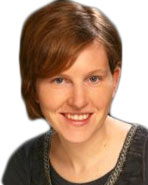
\includegraphics[width=1in,height=1.25in,clip,keepaspectratio]{photos/waltemath.jpg}}]{Dagmar Waltemath}
received her Ph.D. degree in Computer Science from the University of Rostock, Germany in 2011. 
Her research focusses on tools and methods to improve the reproducibility of scientific results obtained from simulation models and in the field of computational biology. 
Dr.~Waltemath is currently a junior research group leader at the Systems Biology and Bioinformatics group at the University of Rostock. 
Her group develops methods for improved model management, model provenance, search and retrieval, and investigates means to integrate model-related information.  
Dr.~Waltemath is an elected COMBINE coordinator and works as an SBML Editor. 
Contact her at dagmar.waltemath@uni-rostock.de
\end{IEEEbiography}

\begin{IEEEbiography}[{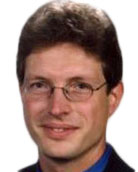
\includegraphics[width=1in,height=1.25in,clip,keepaspectratio]{photos/schreiber.jpg}}]{Falk Schreiber} 
received his Ph.D. degree (2001) and habilitation (2006) in Computer Science both from the University of Passau, Germany. 
He is a professor at Monash University's Faculty of IT and an adjunct professor at Martin Luther University Halle-Wittenberg's Institute of Computer Science. 
His interests are visual computing and visual analytics of biological data, analysis of structure and dynamics of biological networks, integration of multimodal data, standards for systems biology, as well as modeling and analysis of metabolism. 
He served twice as SBGN editor and is a COMBINE coordinator.
Contact him at falk.schreiber@monash.edu.
\end{IEEEbiography}

\begin{IEEEbiography}[{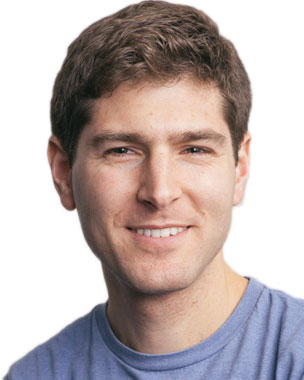
\includegraphics[width=1in,height=1.25in,clip,keepaspectratio]{photos/karr.jpg}}]{Jonathan R. Karr}
received the Ph.D. degree in Biophysics and the M.S. degree in Medicine from Stanford University, Stanford, CA, USA in 2014 and the S.B. degrees in Physics and Brain \& Cognitive Sciences from the Massachusetts Institute of Technology, Cambridge, MA, USA in 2006. 
Dr. Karr is currently a Fellow at the Icahn School of Medicine at Mount Sinai in New York, NY, USA. 
His research focuses on the development of comprehensive whole-cell computational models and their applications to bioengineering and medicine. 
Contact him at jkarr@stanford.edu.
\end{IEEEbiography}

% You can push biographies down or up by placing a \vfill before or after them. The appropriate
% use of \vfill depends on what kind of text is on the last page and whether or not the columns are being equalized.

%\vfill

% Can be used to pull up biographies so that the bottom of the last one is flush with the other column.
%\enlargethispage{-5in}

% ..........................................................................
% End.

\end{document}
